\documentclass[12pt,pdftex,titlepage]{report}

\author{\textbf{Noah Santschi-Cooney}
\\\\\\\small{Final Year Project - BSc in Computer Science}
\\\\\\\small{Jason Quinlan}
\\\\\\\small{Department of Computer Science}
\\\small{University College Cork}}
\title{\textbf{Alternative Visualisations of Distributed Tracing data in a complex, large-scale distributed system}}
\date{\vfill\small{3rd April 2020}}

\usepackage[dvipsnames]{xcolor}
\usepackage[utf8]{inputenc}
\usepackage[english]{babel}
\pagenumbering{roman}

\usepackage{graphicx}
\graphicspath{{./assets/}}

\PassOptionsToPackage{hyphens}{url}\usepackage{url}
\usepackage{microtype, caption, copyrightbox, textcomp, hyperref, listings, assets/listings-golang}
\captionsetup[lstlisting]{font={footnotesize},width=0.8\linewidth}
\captionsetup[figure]{font={footnotesize},width=0.8\linewidth}

\hypersetup{
    colorlinks,
    citecolor=black,
    filecolor=black,
    linkcolor=black,
    urlcolor=black
}
\lstset{
    frame=leftline,
    basicstyle=\scriptsize\ttfamily,
    keywordstyle=\color{Blue},
    numbers=left,
    numbersep=5pt,
    showstringspaces=false, 
    stringstyle=\color{ForestGreen},
    commentstyle=\color{gray},
    tabsize=4,
    language=Go
}

\makeatletter
\def\@makechapterhead#1{%
  \vspace*{20\p@}% <----------------- Space from top of page to Chapter #
  {\parindent \z@ \raggedright \normalfont
    \ifnum \c@secnumdepth >\m@ne
        \huge\bfseries \thechapter.\ % <-- Chapter # (without "Chapter")
    \fi
    \interlinepenalty\@M
    #1\par\nobreak% <------------------ Chapter title
    \vskip 20\p@% <------------------ Space between chapter title and first paragraph
  }}
\makeatother

\begin{document}
    \maketitle    

    \chapter*{Abstract}
        \addcontentsline{toc}{chapter}{Abstract}
        Modern Internet services are often implemented as complex, large-scale distributed systems. These applications are constructed from collections 
        of software modules that could span many thousands of machines across multiple physical facilities. With the rise of modern Micro-service and 
        Service-Oriented designs, traditional tooling used to monitor application behaviour is no longer viable, especially at scale. 
        
        To understanding the flow and life cycle of a unit of work performed in multiple pieces across various components in a distributed system, the concept of 
        Distributed Tracing was born. Distributed Tracing was first introduced to the mainstream world in 2010 after the publication of Google’s Dapper
        paper. Since then, various vendors have come out with their own Dapper-inspired services, most of them based off flame or timeline graphs. 
        
        The goal of this project is dual-faceted:
        \begin{itemize}
            \item Explore and research possible alternative uses and visualisation methods utilising data collected from distributed tracing clients.
            \item Implement one or more of the proposed alternatives.
        \end{itemize}

    \chapter*{Declaration of Originality}
        \addcontentsline{toc}{chapter}{Declaration of Originality}
        In signing this declaration, you are confirming, in writing, that the submitted work
        is entirely your own original work, except where clearly attributed otherwise, and
        that it has not been submitted partly or wholly for any other educational award. I
        hereby declare that:
        \begin{itemize}
            \item this is all my own work, unless clearly indicated otherwise, with full and proper accreditation;  
            \item with respect to my own work: none of it has been submitted at any educational institution contributing in any way to an educational award;
            \item with respect to another’s work: all text, diagrams, code, or ideas, whether verbatim, paraphrased or otherwise modified or adapted, 
            have been duly attributed to the source in a scholarly manner, whether from books, papers, lecture notes or any other student’s work, whether
            published or unpublished, electronically or in print.
        \end{itemize}   
        \vspace{10mm}
        Signed: \dotfill
        \\\\
        Date: \dotfill

    \chapter*{Acknowledgements}
        \addcontentsline{toc}{chapter}{Acknowledgements}
        
    \tableofcontents

    \chapter{Introduction}
    \pagenumbering{arabic}
    \setcounter{page}{1}
        \section{Problem}
            Within the last decade, the way modern applications are being built and deployed has changed dramatically. With the shift from collocation to cloud computing,
            virtual machines to containerization technologies, monoliths to micro-services and beyond, software developers have been able to adjust to 
            the monotonical increase in internet traffic, shipping highly scalable, efficient and reliable software that meets the ever-demanding needs of their customers
            with the slew of emerging technologies.

            While this shift has undoubtedly solved many issues with regards to scaling services in terms of both maintainability as feature sets increase and in keeping up
            with an every larger number of online users, it has introduced a whole new suite of problems that needed to be addressed in terms of reliability and application 
            monitoring. With the splitting of monolithic applications into micro-services, the failure points are extended to issues in the network, including but not limited
            to network congestion, DNS resolution errors etc. Developers are ever more inclined to code failure resilience into their applications, falling back gracefully in 
            apprehension of unforeseeable failures.

            As these new distributed system architectures evolved and became ever more widespread, traditional application monitoring tools consistently fell short of providing
            developers and systems operators with the means to gain introspection into systems and their failures in production scenarios. Traditional monolithic systems often
            utilized logging and metrics to gain introspection into the application and for alerting on rules respectively. For such systems, these process-scoped measures often 
            provided good insight into a system, correlating logs on their thread identifier/name as each thread would handle a single request sequentially. As these systems 
            adopted asynchronous execution models, where a request's lifetime may not be confined to a single thread, the previous approach no longer works, making observing
            the behaviour of such systems very difficult unless developers annotated logs with request-scoped identifiers. The final evolution of concurrency in application systems is
            commonly referred to as \textit{distributed concurrency}. This is often associated with micro-services, in which a request is no longer constrained to being executed
            in a single process, but may span multiple processes and even servers. Figure~\ref{fig:concurrency} highlights this evolution, from simple, single threaded applications,
            through to micro-service-like architectures.

            \begin{figure}[htb!]
                \centering
                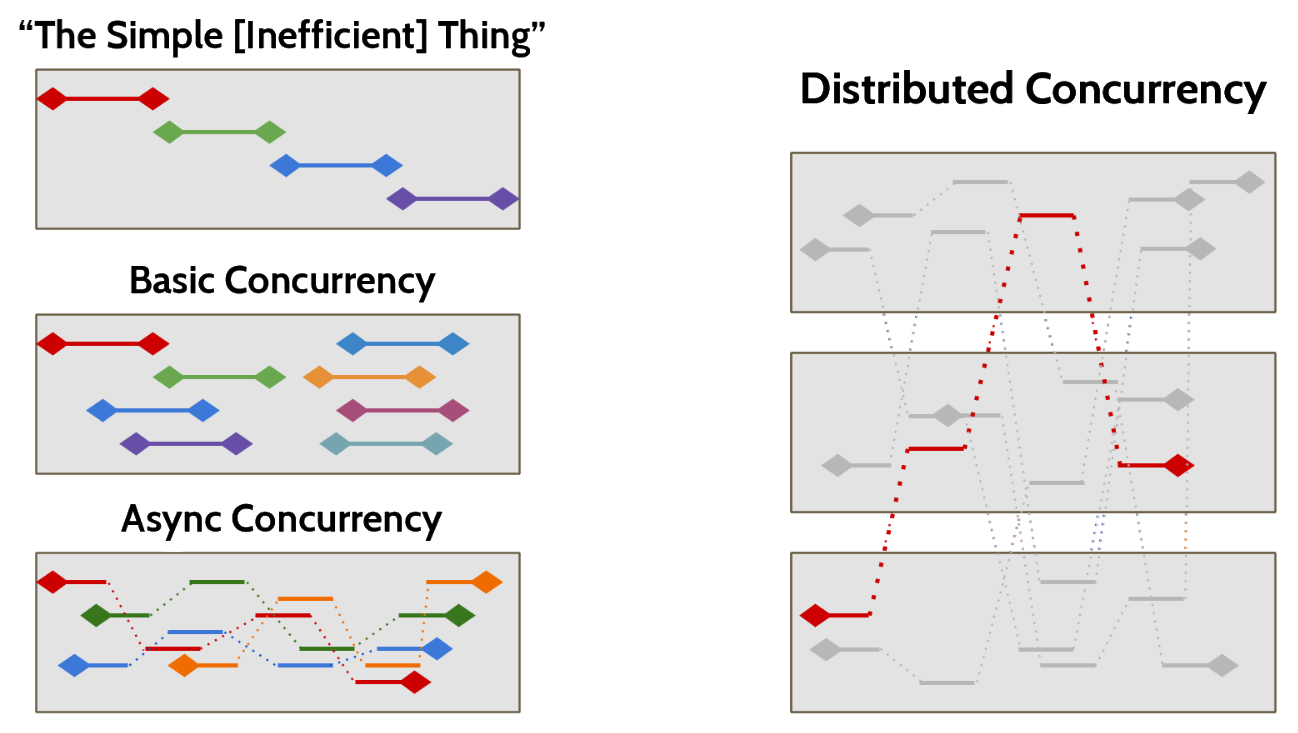
\includegraphics{concurrency.png}
                \caption{Evolution of concurrent systems.}
                \label{fig:concurrency}
            \end{figure}
        
        \section{Debuggers}
            In traditional single process applications, debugger tools, both standalone and bundled with integrated development environments (IDEs), are invaluable in their
            use of isolating bugs in codebases of any size. They have the capability to give complete overview of stack and heap allocated variables as well as being able to set
            breakpoints to step through code. Figure~\ref{fig:debugger} highlights the various insights and utilities provided by such tools, including the display of call stacks,
            local and global variables as well as various utilities to step through code at the line and function levels.

            \begin{figure}[hbt!]
                \centering
                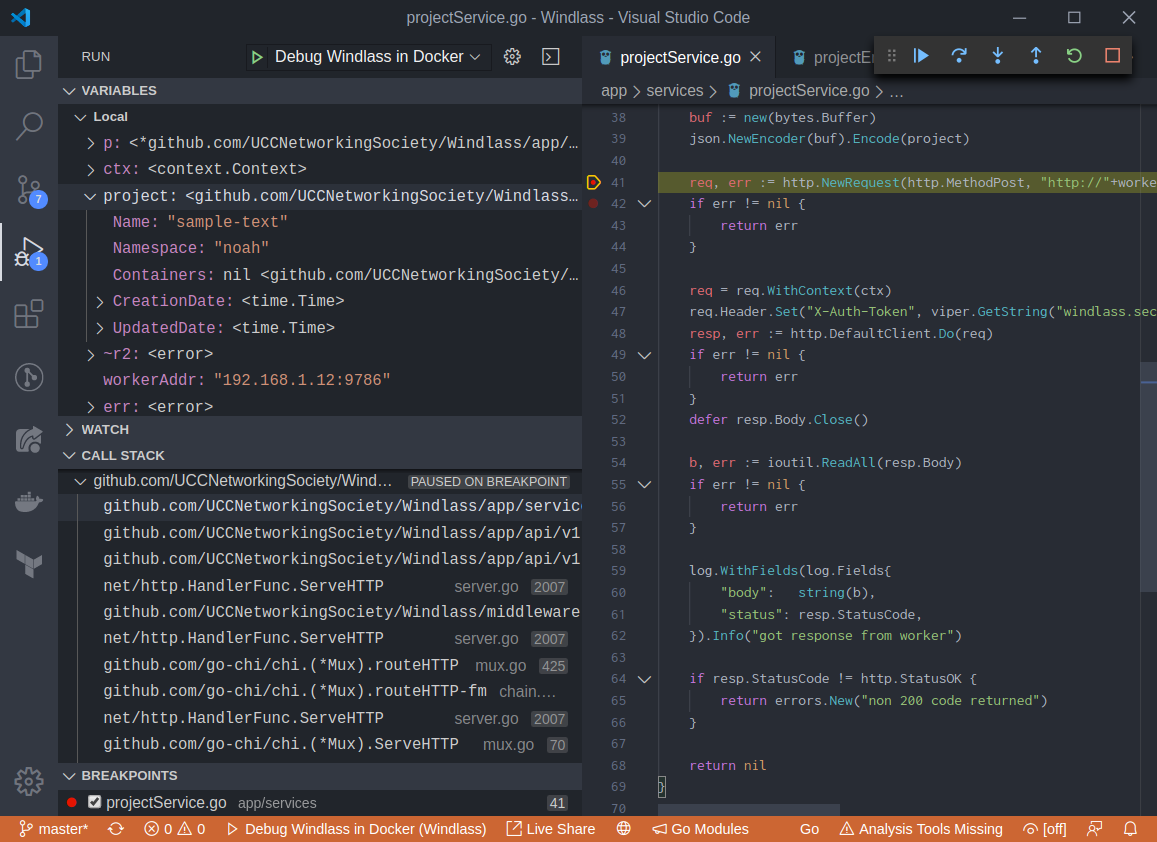
\includegraphics[scale=0.335]{debugger}
                \caption{Screenshot of the Visual Studio Code debugger in action. Clockwise, shown are an expandable list of local and global variables, the currently open file view
                with the line currently halted on highlighted along with controls for stepping and finally the function call stack.}
                \label{fig:debugger}
            \end{figure}
            
            However, it's often infeasible to use them in production scenarios due to their nature of halting complete execution of the process.
            This makes it unsuitable for debugging issues that manifest in production that developers are finding it difficult to reproduce in development scenarios, as is often
            a common scenario due to subtle parity differences between development and production systems.

        \section{Distributed Tracing}
            As traditional tooling is not designed to accommodate for this distributed concurrency system, new methodologies were needed to regain observability into the systems.
            Observing single systems individually, as was done with traditional tooling, no longer painted the full picture of a request as it travels through multiple system 
            components. Distributed tracing systems and platforms build upon the concepts of reconstructing a request from a series of event streams from each component involved
            in the request, with distributed context propagation and aggregation, building causality graphs from a request-centric point of view.

            \begin{figure}[hbt!]
                \centering
                \copyrightbox[r]{
                    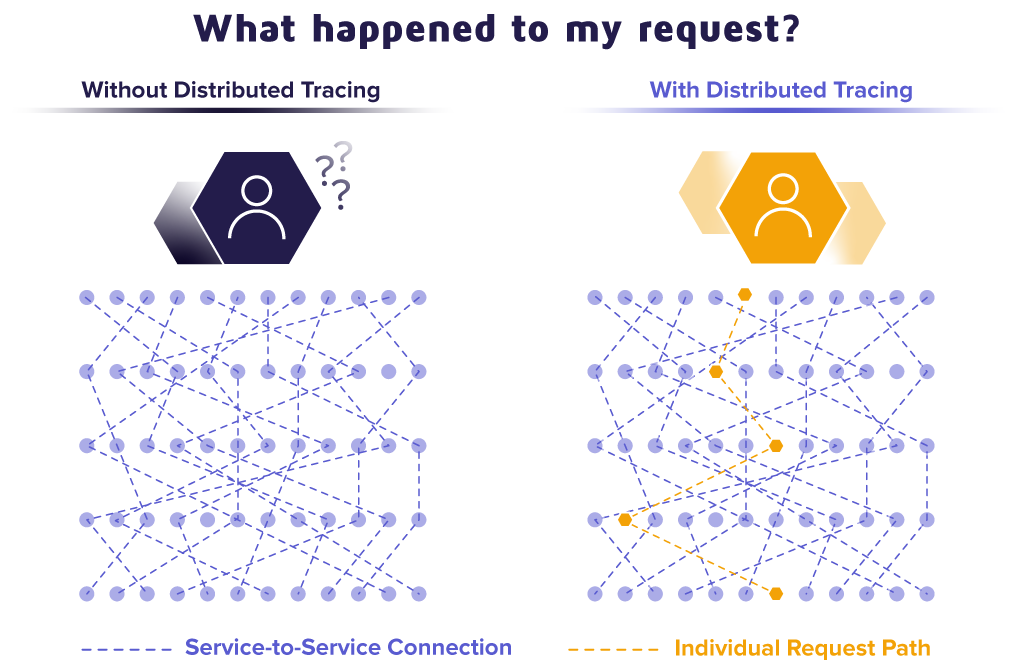
\includegraphics[scale=1.7]{distributed}
                }{
                    \tiny{\textcopyright Nic Munroe "Hit the Ground Running with Distributed Tracing Core Concepts" on Medium}
                }
                \caption{Depiction of a complex distributed system with much inter-connectivity between services.}
                \label{fig:dist}
            \end{figure}

            Code is instrumented at various points of interest, recording annotated events with metadata such as the user ID associated with the request, SQL statements being 
            executed on a database etc. These events are often shipped to a collector/exporter, from which they are either stored in a database or sent to a hosted vendor, such as
            LightStep or Honeycomb, after which they can be queried, retrieved and displayed.

        \section{Motivation \& Goals}
            As distributed tracing is still a relatively new idea and only as of recently gathering mainstream interest in the industry, research and advancements on the topic are 
            as of yet still sparse. Current vendors often provide a limit set of capabilities and operations that can be performed on the data output from instrumented distributed systems,
            most commonly simple expandable \textit{gantt charts} or, less commonly, simple, mostly static, service dependency graphs that offer little value and utility.

            To further research in this field, the project will attempt to explore alternative and hopefully improved ways of consuming and presenting the data from instrumented
            applications. Two ideas were planned to be explored and, if possible, implemented as proof of concepts:

            \begin{itemize}
                \item Advancements in Service Topology/Dependency graphs
                \item Editor Debugger integration                
            \end{itemize}

            % TODO:
            The viability and findings of both explored options will be discussed, with performance benchmarks where relevant being presented to highlight the feasibility of different
            approaches 

        \section{Project Summary}
            This project builds upon the concepts of distributed tracing, exploring ways to provide novel and high-value derivable ways of visualizing and presenting distributed tracing
            data to developers. Modern standards, tools and integrations will be utilized to test the viability of less common and unexplored visualizations of distributed tracing data.

            In Chapter 2, the history of distributed tracing will be introduced, while also covering some common vocabulary relevant to the topic and where they originated. It will also
            cover some of the standards that this project builds around. In Chapter 3, the project architecture design choices will be discussed and how they impacted the project, ranging
            from the frontend frameworks chosen to the backend API and supporting services that power the various implementations. Finally, the different visualizations will be evaluated
            on the value the provide as well as the feasibility of utilizing them in real-world scenarios. Chapters 5 and 6 will draw the writeup to a conclusion, detailing the closing
            thoughts and putting forward ideas for future work on the ideas explored in this project.

    \chapter{Background}
        \section{History}
            \subsection{Dapper}
                Released in April 2010, Google published a paper describing the design decisions behind an in-house implementation 
                of distributed tracing, named Dapper. It is commonly believed that this paper describes the common ancestor to 
                many tools that implement a form of distributed tracing.

                The Dapper paper introduces some of the core primitives that underpin modern day standards. Most notable are the concepts
                of a directed acyclic graph (DAG) called a \textit{trace tree} and its nodes, which are referred to as \textit{spans}. 
                The trace tree forms a relationship between spans, not unakin to a tree of stack frames that may be generated by
                gathering stack frames over time, albeit generally at a much higher level than at the level of individual subroutine calls. 

                Figure~\ref{fig:dappertrace} illustrates a trace tree with five spans. Each span is shown to contain 3 specific pieces of
                metadata alongside the start and end timestamps necessarily to reconstruct the temporal relationships: a human-readable
                \textit{span name}, an integer \textit{span ID} and an integer \textit{parent ID}. The latter two
                data points are used to reconstruct the relationship between individual spans. A span without a parent ID becomes the 
                \textit{root span} of a trace tree. Not shown is another important but, as of right now, not relevant piece of metadata, the 
                \textit{trace ID}, which is common amongst all spans within a single trace tree.

                \begin{figure}[htb!]
                    \centering
                    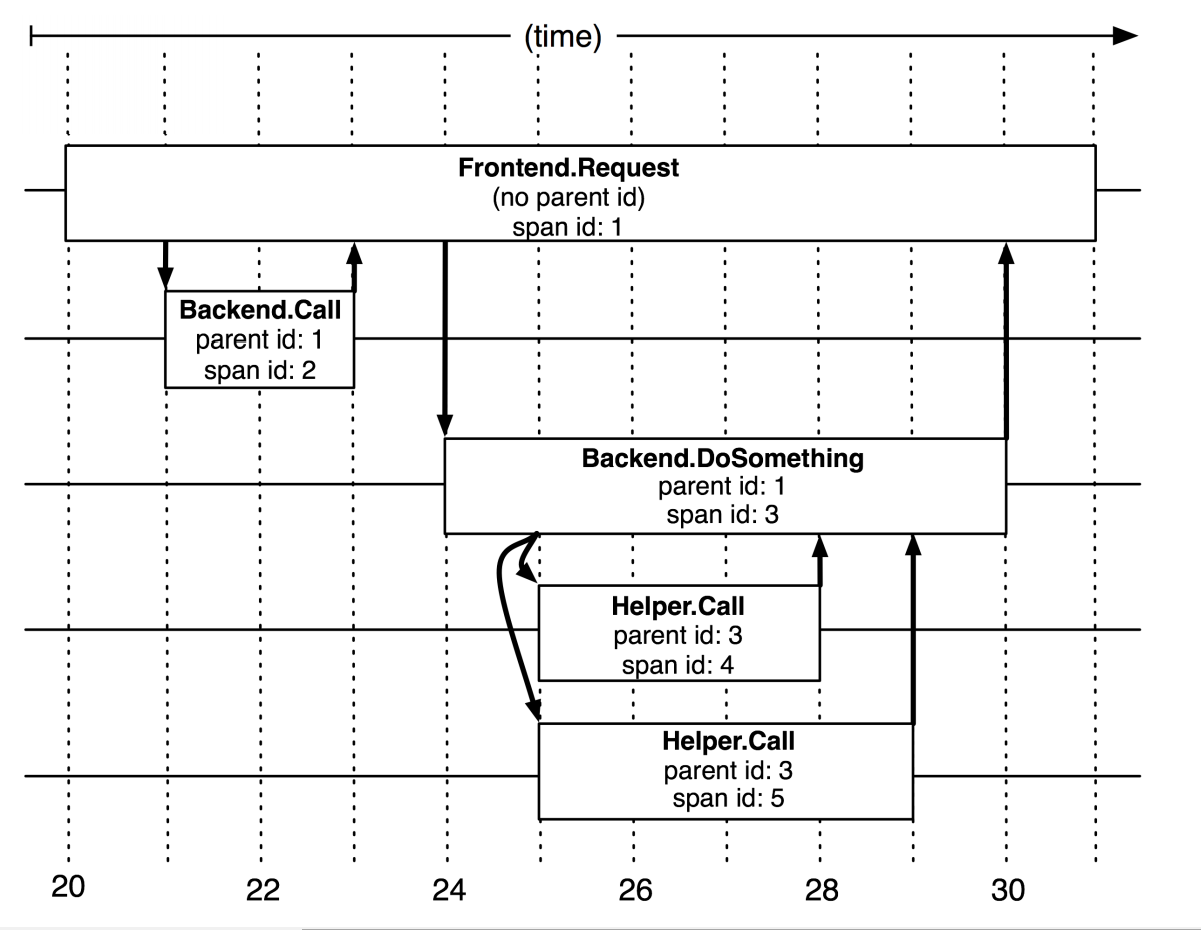
\includegraphics[scale=1]{dappertrace}
                    \caption{The relationships between traces in a trace tree.}
                    \label{fig:dappertrace}
                \end{figure}

                As described thus far, Dapper trace trees allow for a detailed view of the relationships of distributed systems within
                Google. When using this data for debugging or performance analysis, it can often be convenient or even necessary to 
                have additional context surrounding a trace tree or its individual spans. As such, the paper describes a simple API 
                through which application developers can provide a combination of two types of annotations: timestamped textual annotations
                and key-value, allowing for defining arbitrary equivalence classes between traces which can be operated upon in the analysis
                tools.

            \subsection{OpenTracing}
                OpenTracing\cite{opentracing} project's inception came about in October 2015, it has since become a project under the 
                Cloud Native Computing Foundation in 2016, created to standardize a set of vendor neutral and programming language agnostic
                application programming interfaces (APIs) for instrumenting code for distributed tracing. Heavily inspired by the Dapper
                paper, it borrows many of the nouns and verbs outlined in the Dapper paper, including \textit{traces} and \textit{spans}.
                Dapper's timestamped annotations are referred to as \textit{logs} in the OpenTracing specification, while the key-value pairs
                are named \textit{tags}. 

                The OpenTracing API also specifies how a trace cross process boundaries, so that spans created in different processes can be
                associated with a common trace tree. This was named the \textit{span context} and at it's most basic level contains the 
                overlying trace ID as well as the current span ID. With this, new spans generated across process boundaries have the ability to
                to specify their parent span as well as their common trace, without propagating an entire span, which may prove costly as more
                tags and logs are attached to a span.

                Figure~\ref{fig:opentracing} shows a timeline based visualization of where the different components of the OpenTracing API interface are utilized in
                the larger picture of creating a span through use of distributed context propagation in the span context

                \begin{figure}[hbt!]
                    \centering
                    \copyrightbox[r]{
                        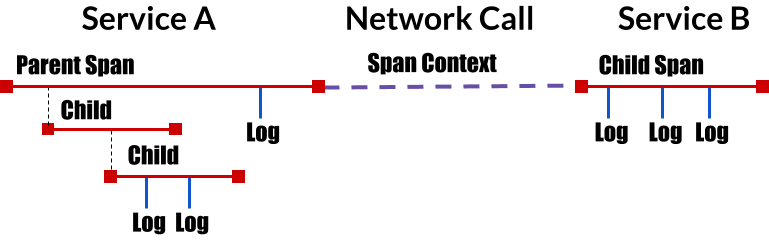
\includegraphics[scale=0.5]{opentracing}
                    }{\tiny{\textcopyright OpenTracing "OpenTracing Overview"}}
                    \caption{Infographic visualizing the different components that make up the OpenTracing API interface and how they relate to different services
                    and the network}
                    \label{fig:opentracing}
                \end{figure}

                As there are multiple output sinks which can consume OpenTracing data, from self hosting services such as Jaeger to hosted vendors like LightStep, and given that
                different platforms may have different, vendor-specific options for operations such as access control, authorization etc, vendors provide different mechanisms
                and attributes for creating instances of OpenTracing API \textit{tracers} implementations.

% Latex expects everything on one indentation level? very sad
                \begin{lstlisting}[caption={Example Golang snippet of instatiating a Datadog OpenTracing compatible tracer.}]
package main

import (
    "gopkg.in/DataDog/dd-trace-go.v1/ddtrace"
    "gopkg.in/DataDog/dd-trace-go.v1/ddtrace/opentracer"
    "github.com/opentracing/opentracing-go"
)

// Start a Datadog tracer, optionally providing a set of options,
// returning an opentracing.Tracer which wraps it.
t := opentracer.New(
    tracer.WithAgentAddr("host:port"),
    tracer.WithServiceName("sample-text"))

    // Use it with the OpenTracing API, setting it as global.
opentracing.SetGlobalTracer(t)
                \end{lstlisting}

                \newpage
                \begin{lstlisting}[caption={Example Golang snippet of instatiating a Jaeger OpenTracing compatible tracer.}]
package main

import (
    "github.com/uber/jaeger-client-go"
    "github.com/uber/jaeger-client-go/transport"
    "github.com/opentracing/opentracing-go"
)

// Start a Jaeger tracer, supplying the sampling strategy and the
// reporter configuration.
t, closer := jaeger.NewTracer(
    "sample-text",
    jaeger.NewConstSampler(true),
    jaeger.NewRemoteReporter(transport.NewHTTPTransport("host:port")))
defer closer.Close()

// Use it with the OpenTracing API, setting it as global.
opentracing.SetGlobalTracer(t)                    
                \end{lstlisting}

            \subsection{OpenTelemetry}
                The OpenTelemetry\cite{opentelemetry} project came about as a result of the merging of two previous projects, namely the previously mentioned OpenTracing
                project as well as OpenCensus project. The OpenCensus project originated from Google and had many similar goals to OpenTracing. Alongside having an interface
                for distributed tracing gathering, it also supported instrumenting applications to output application metrics data. To reduce the fragmentation in having
                two independent APIs for distributed tracing, the two projects decided to merge into one standard going forward. At the time of writing, support for OpenTelemetry
                is still very sparse, due to the fact that it is still a very new specification set, while still being largely backwards compatible with both OpenTracing and 
                OpenCensus, providing API bridges to maintain compatibility. 

                The OpenTelemetry API improves upon OpenTracing by introducing a set specification for context propagating header keys used to identify specific values, created
                as a W3C specification. In OpenTracing API implementations, different vendors would use different keys to denote values such as the trace ID etc in, for example, 
                HTTP headers. This would break the context chain if different codebases used different vendor implementations in a service dependency graph. By demoting vendor
                libraries to providing simple \textit{exporters} that define how distributed tracing data is exported to backend systems rather than having them provide
                tracer implementations like the way it was done with the OpenTracing API, the OpenTelemetry project achieves a better level of interoperability between codebases, 
                where the OpenTelemetry \textit{collector} can act as the common sink for the different services, becoming the source of truth regarding the eventual backend system
                to which the distributed tracing data will be exported to.

                \begin{figure}[hbt!]
                    \centering
                    \copyrightbox[r]{
                        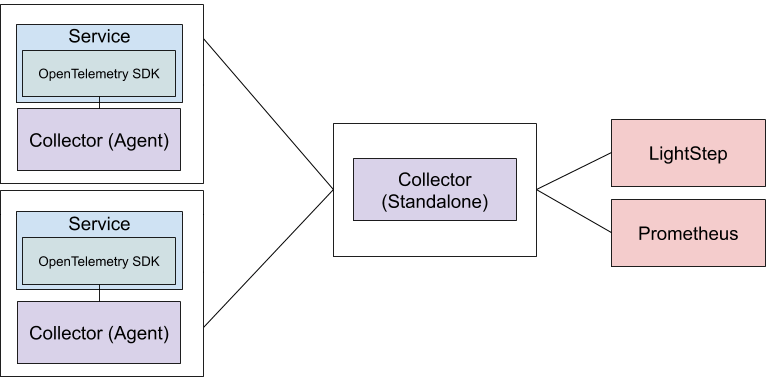
\includegraphics[scale=0.5]{opentelemetry-exporter}
                    }{\tiny{\textcopyright{LightStep "OpenTelemetry 101: What is an Exporter?"}}}
                    \caption{A high level overview of a typical OpenTelemetry setup, with services hooking into the OpenTelemetry SDK to output telemetry to
                    OpenTelemetry Collectors, which themselves forward data to the standalone Collector sink, which is configured to send metrics to a \textit{Prometheus}
                    server and distributed tracing data to the LightStep API.}
                    \label{fig:otexporter}
                \end{figure}
                

    \chapter{Design \& Implementation}
        \small{In this section, the different technical aspects will be covered, design decisions and components that played a role throughout the projects lifecycle.
        This will include third party services and the roles they played.}

        \section{Architecture Design}
            \subsection{Distributed Tracing API}
                The OpenTracing API interface was chosen as the foundation for this project. This decision was made due to the large language support and comprehensive open
                source tooling built around the OpenTracing API. It is also widely supported by many third party vendors, including LightStep, DataDog and Honeycomb amongst 
                numerous others.

                OpenTelemetry was initially considered as an alternative choice instead of OpenTracing, but was ultimately decided against due to it still being a very new
                standard, with OpenTracing having much more comprehensive support and documentation resources from both application libraries and distributed tracing tools.
                This lowered the productivity barrier, as the OpenTelemetry backing components, including the collector, introduce more complexity than what exists in a simple
                development-oriented OpenTracing setup.

                Potential explorations around the OpenTelemetry API are discussed in the \textit{Future Work} section.

            \subsection{Supporting Services}
                As both explored ideas will be interacting with distributed tracing data, there are two pieces to the puzzle of having a set of traces to work with.
                Firstly, a way of collecting trace data from applications is needed, and secondly, the database into which the data is persisted.
                
                The OpenTracing platform, Jaeger, was chosen for this project. Jaeger is wholly self-hostable, providing a convenient setup for single-machine development purposes with
                a single, all-inclusive binary available from the distribution archives, as well as a pre-built \textit{Docker} image published to DockerHub. The full Jaeger package,
                available in whole in the aforementioned all-inclusive formats, includes the trace collector, trace search and visualization user interface and agent.

                By default, the all-in-one Jaeger distribution stores all trace data in-memory. For convenience to persist data in between machine reboots, the JSON document search engine
                database, \textit{Elasticsearch}, was chosen as the storage backend for Jaeger, as one of two possible choices alongside \textit{Apache Cassandra}, a column store document
                database. The Backend API, discussed later in this chapter, interfaces with the Elasticsearch database as the source of truth for the trace data. A complementary user interface
                for Elasticsearch, maintained by the developers of Elasticsearch, \textit{Kibana}, was used throughout the development of the project to view the raw trace data as it is 
                represented in the database.

                In line with how the OpenTracing API works, the Jaeger language-specific instrumenting libraries must be used to inject the Jaeger tracer implementation into the 
                applications.


            \subsection{Backend API}
                GraphQL vs Rest
                ES lib
                Kotlin
                
        \section{Implementations}
                
            \subsection{Backend API}

            \subsection{Service Topology Frontend}

            \subsection{Debug Adapter}

    \chapter{Evaluation}
    
    \chapter{Conclusion \& Future}
        \section{Conclusion}

        \section{Future Work}
            \subsection{OpenTelemetry}

    \begin{thebibliography}{69}
        \addcontentsline{toc}{chapter}{Bibliography}    

        \bibitem{dapper}
        Benjamin H. Sigelman, Luiz André Barroso, Mike Burrows, Pat Stephenson, Manoj Plakal, Donald Beaver, Saul Jaspan, Chandan Shanbhag, \\
        \textit{Dapper, a Large-Scale Distributed Systems Tracing Infrastructure.} \\
        Google, Inc. 2010 \\
        \url{https://research.google/pubs/pub36356/}

        \bibitem{mbta}
        Mike Barry, Brian Card, \textit{Visualizing MBTA Data.}
        10th June 2014 \\
        \url{https://mbtaviz.github.io/}

        \bibitem{opentracing}
        Benjamin H. Sigelman (co creator), \textit{The OpenTracing project.}
        October 2015 \\
        \url{https://opentracing.io/}

        \bibitem{opentelemetry}
        OpenTelemetry Authors, \textit{The OpenTelemetry Project.} 
        19th April 2019 \\
        \url{https://opentelemetry.io/}
    \end{thebibliography}
\end{document}